\documentclass[conference]{IEEEtran}
\IEEEoverridecommandlockouts
% The preceding line is only needed to identify funding in the first footnote. If that is unneeded, please comment it out.
\usepackage[utf8]{inputenc}
\usepackage[T1]{fontenc}
\usepackage{cite}
\usepackage{amsmath,amssymb,amsfonts}
\usepackage{algorithmic}
\usepackage{graphicx}
\usepackage{textcomp}
\usepackage{xcolor}
\usepackage{booktabs}
\usepackage{siunitx}
\sisetup{per-mode=symbol}
\usepackage{tikz}
\usetikzlibrary{arrows.meta,positioning,calc,fit,backgrounds}
\graphicspath{{figs/}}

\def\BibTeX{{\rm B\kern-.05em{\sc i\kern-.025em b}\kern-.08em
    T\kern-.1667em\lower.7ex\hbox{E}\kern-.125emX}}

% ============================================================================
% NOTE FOR THE AUTHORS
%  - Figures are in ./figs/ (already copied from the project's images/ folder).
%  - Search for "PLACEHOLDER" to find the spots where the validated force-PI
%    data of the arm (curves + metrics) must be inserted (Section Results).
%  - Fill in the five authors below.
% ============================================================================

\begin{document}

\title{A Digital Twin of a Collaborative Manipulator for Closed-Loop Force-Controlled Tactile Palpation}

% ---- TODO: complete co-authors 2-5 (advisor, collaborators) -----------------
\author{%
\IEEEauthorblockN{1\textsuperscript{st} Lucas Martins Primo}
\IEEEauthorblockA{\textit{Faculdade de Engenharia El\'etrica} \\
\textit{Universidade Federal de Uberl\^andia}\\
Uberl\^andia, Brazil \\
ORCID: 0009-0001-6129-0852}
\and
\IEEEauthorblockN{2\textsuperscript{nd} Given Name Surname}
\IEEEauthorblockA{\textit{dept. name of organization} \\
\textit{name of organization}\\
City, Country \\
email or ORCID}
\and
\IEEEauthorblockN{3\textsuperscript{rd} Given Name Surname}
\IEEEauthorblockA{\textit{dept. name of organization} \\
\textit{name of organization}\\
City, Country \\
email or ORCID}
\and
\IEEEauthorblockN{4\textsuperscript{th} Given Name Surname}
\IEEEauthorblockA{\textit{dept. name of organization} \\
\textit{name of organization}\\
City, Country \\
email or ORCID}
\and
\IEEEauthorblockN{5\textsuperscript{th} Given Name Surname}
\IEEEauthorblockA{\textit{dept. name of organization} \\
\textit{name of organization}\\
City, Country \\
email or ORCID}
}

\maketitle

\begin{abstract}
This paper presents a digital-twin platform of a six degree-of-freedom
collaborative manipulator for closed-loop, force-controlled tactile palpation in
a biomedical context. A kinematically faithful simulation of a Dobot CR10 arm,
running under ROS 2 and Gazebo, is coupled to the physical robot through a
real-time mirroring link, so that the same control software drives both the
virtual and the real arm. A force-instrumented contact tool, mounted on a
uniaxial load cell, reproduces the robotic palpation protocol of Gupta et al.:
the end effector approaches a surface, regulates the normal contact force to a
selectable set point, holds until the force stabilizes, slides laterally at
constant speed, and retracts. Force regulation uses an outer proportional-integral
loop that converts the contact-force error into a Cartesian approach velocity,
mapped to joint motion through a damped least-squares Jacobian and streamed at
33 Hz. We describe the twin, its kinematics, the finite-state palpation protocol,
the force-control law expressed as a tunable admittance, the safety layer that
bounds contact forces, and the force-tracking metrics used to characterize the
closed-loop response. The platform provides a safe, repeatable environment for
developing tactile-exploration behaviors before deployment on the physical
system.
\end{abstract}

\begin{IEEEkeywords}
digital twin, force control, tactile palpation, collaborative robot, ROS 2,
Gazebo, biomedical robotics, tactile exploration
\end{IEEEkeywords}

\section{Introduction}
Touch is central to how humans explore and manipulate the world, and restoring
or emulating it is a recurring goal in assistive and surgical robotics
\cite{gupta2021,konstantinova2014}. Tactile palpation, pressing and sliding a
probe against a surface under controlled normal force, is the canonical motion
used to estimate surface and sub-surface properties such as texture, stiffness,
and the presence of inclusions \cite{konstantinova2014}. Reproducing this
behavior reliably on a robot requires accurate kinematics, a well-tuned
force-control loop, and a safe development environment, because uncontrolled
contact forces can damage both the specimen and the hardware.

This work develops a tactile palpation station built on a Dobot CR10
collaborative arm. A force-instrumented contact tool, attached to
a uniaxial load cell, reproduces the robotic palpation protocol of Gupta et al.
\cite{gupta2021}: contact, hold, slide, and retract, with the normal force held
constant by closed-loop control. We deliberately focus, in this paper, on the
\emph{manipulator side} of that protocol (the digital twin and its
force-control loop) rather than on tactile transduction.

\textbf{Digital twin.} The core of the contribution is a \emph{digital twin} of
the manipulator: a simulation that is geometrically and kinematically faithful
to the physical arm and that is connected to it by a real-time, bidirectional
link. The twin is not merely a visualizer. The same control code runs against
the simulated and the real arm; the simulation can mirror the physical robot's
motion (and vice versa), and real contact-force measurements are fed back into
the loop. This makes the twin a safe, repeatable proving ground in which
force-controlled palpation behaviors are developed, tuned, and validated before
they ever touch a real specimen.

\textbf{Contributions.} The paper (i) describes a ROS~2 / Gazebo digital twin of
a CR10 collaborative arm with a bidirectional sim-to-real link; (ii) details a
finite-state palpation protocol reproducing the Gupta et al. choreography on a
force-instrumented contact tool; (iii) presents a streaming
proportional-integral (PI) force-control law that regulates the normal contact
force through a damped least-squares Jacobian at \SI{33}{\hertz}; and (iv)
reports the closed-loop force-tracking performance of the arm together with the
safety layer that bounds contact forces.

\section{Related Work}
\textbf{Robotic tactile palpation.} Tactile exploration for property estimation,
including stiffness mapping and tumor localization in minimally invasive
surgery, has been widely studied \cite{konstantinova2014,beccani2014}. The protocol we
reproduce was introduced by Gupta et al. \cite{gupta2021}, who mounted a
force-instrumented end effector on a UR-10 arm and executed a four-phase
contact/hold/slide/retract cycle with the normal force regulated to
\SI{1}{\newton} in closed loop, sliding at $5$, $10$, and \SI{15}{\milli\meter
\per\second}. Their study targets neuromorphic texture classification; here we
re-implement the \emph{robotic palpation protocol} of that work, its motion and
force choreography, as a digital twin, and we study the force-regulation
behavior of the arm.

\textbf{Force control.} Regulating interaction forces between a manipulator and
its environment is a classical problem \cite{siciliano2009,hogan1985,villani2016}. Pure
position control is unsuitable for contact tasks; impedance and admittance
schemes shape the dynamic relationship between motion and force
\cite{hogan1985}. Our load cell measures only the normal force along the
approach axis, so we adopt an explicit outer force loop that produces a Cartesian
velocity correction along that axis, an admittance-like scheme layered on top of
the arm's position-controlled joints.

\textbf{Digital twins and simulation.} ROS~2 \cite{macenski2022} and Gazebo
\cite{koenig2004} are the de-facto open-source stack for robot simulation and
control. Digital twins extend simulation with a live, bidirectional coupling to
the physical asset \cite{grieves2017,tao2019}. Kritzinger et al.
\cite{kritzinger2018} distinguish a digital \emph{model} (manual data flow), a
digital \emph{shadow} (automatic real-to-virtual flow), and a digital \emph{twin}
(automatic flow in both directions). Our system realizes this bidirectional flow
in its \textsc{mirror} mode (Section~\ref{sec:mirror}): the controller streams
joint set points to the physical arm and to the simulation simultaneously, while
the real load-cell force is fed back to close the control loop. A separate
\textsc{sim\_only} mode drives the simulation alone, for collision-free rehearsal
of motions before they are run on the robot. Both build on ROS~2 Humble and
Gazebo Classic with identical controllers and kinematics in the two worlds.

\textbf{Biomedical motivation.} Controlled tactile interaction underlies medical
and assistive applications, from tissue characterization to restoring touch in
upper-limb assistive devices \cite{antfolk2013}. A faithful digital twin of the
manipulator offers a low-risk environment in which such force-controlled contact
behaviors are developed and validated before deployment.

\section{System Overview}
\label{sec:system}
The platform runs on Ubuntu~22.04 with ROS~2 Humble and Gazebo Classic~11, and is
implemented as open ROS~2 packages.\footnote{Source code and configuration:
\texttt{github.com/Martins-Lucaas/RoboticArm}} The
robotic asset is a Dobot CR10 six-axis collaborative arm (Fig.~\ref{fig:hardware};
reach \SI{1375}{\milli\meter}, payload \SI{10}{\kilo\gram}), commanded through its
TCP/IP interface and, in simulation, through a Joint Trajectory Controller (JTC). The arm's URDF is taken from the official Dobot
description package, so the simulated kinematics matches the physical robot.

\begin{figure}[t]
  \centering
  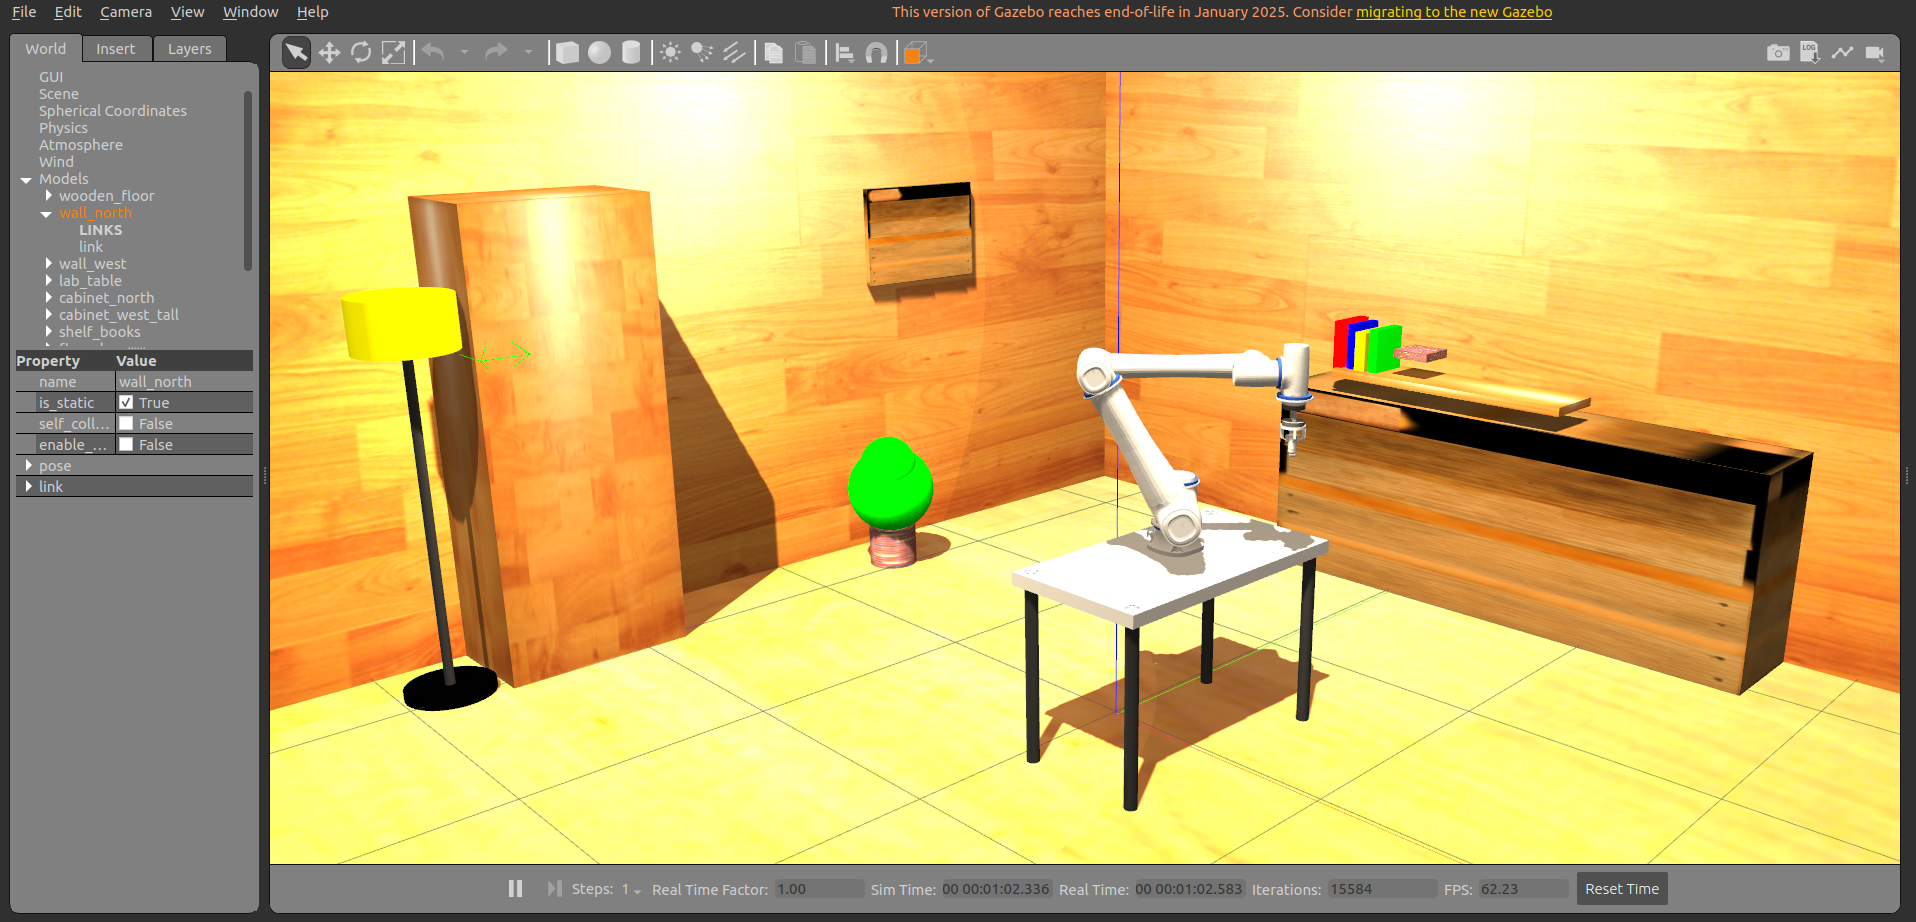
\includegraphics[width=\columnwidth]{touch_pack_gazebo_tactile_cell.png}
  \caption{Digital twin of the palpation cell in Gazebo Classic. The CR10 arm
  carries the force-instrumented \texttt{touch\_tool} over the palpation table.
  The same scene is kinematically identical to the physical robot and, in the
  MIRROR mode of operation, is coupled to it in real time.}
  \label{fig:gazebo}
\end{figure}

\begin{figure}[t]
  \centering
  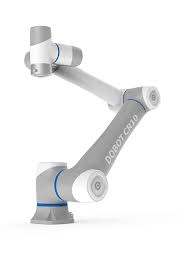
\includegraphics[height=3.4cm]{dobot_cr10_product_photo.jpeg}
  \caption{The physical Dobot CR10 collaborative arm, the real asset mirrored in
  real time by the digital twin (Fig.~\ref{fig:gazebo}). The palpation end
  effector is the force-instrumented contact tool of
  Section~\ref{sec:endeffector}.}
  \label{fig:hardware}
\end{figure}

\subsection{End effector: the force-instrumented contact tool}
\label{sec:endeffector}
The palpation end effector is a \SI{20}{\milli\meter}$\times$\SI{20}{\milli
\meter} square contact tool (\texttt{touch\_tool}) screwed onto a uniaxial load
cell, itself coupled to the arm flange through a printed adapter stack. The tool
center point (TCP) lies \SI{188.5}{\milli\meter} along the flange $z$ axis,
through the coupling chain
flange~$\rightarrow$~lower~coupling~$\rightarrow$~load~cell~$\rightarrow$~upper
coupling~$\rightarrow$~tool. This rigid, single-axis probe is the natural analog
of the single sensorized finger in \cite{gupta2021} and is what closes the
force loop in this paper.

\subsection{Load cell and force feedback}
Contact force is measured by an IP66 aluminum single-point strain-gauge load cell
(sensitivity \SI{2.0}{\milli\volt\per\volt}, combined error \SI{0.03}{\percent} of
full scale, permissible overload \SI{150}{\percent} of full scale), digitized by an
ESP32 microcontroller that samples at \SI{1}{\kilo\hertz} and transmits batched
samples over UDP (about one hundred datagrams per second). Used in its
\SI{5}{\kilo\gram} range (full scale near \SI{49}{\newton}), the
\SI{0.03}{\percent} combined error corresponds to about \SI{0.015}{\newton}, an
order of magnitude below the \SI{0.15}{\newton} HOLD tolerance, so the sensor
accuracy does not limit force regulation. On the host, the
firmware's affine voltage transform is inverted and a per-session calibration
(slope and intercept, obtained by linear regression over known masses) converts
voltage to newtons. A tare step yields the net contact force published on
\texttt{/load\_cell/force\_net}, with the sign convention that compression is
positive and tension is negative. This signal is the feedback variable of the
force-control loop; since it comes from the physical cell, the force loop is
closed in \textsc{mirror} operation (Section~\ref{sec:mirror}).

\subsection{Modes of operation and the sim-to-real link}
\label{sec:mirror}
The twin runs in three modes. In \textsc{sim\_only} the controller drives the
Gazebo arm alone. In \textsc{mirror} the joint set points published by the
controller are simultaneously sent to the physical CR10: during a palpation the
real arm is driven by \texttt{ServoJ} at \SI{33}{\hertz} (minimal latency for
force control), while in idle jogging it follows \texttt{MovJ} commands. A
\emph{drag-teach} facility reverses the direction of the link: the operator
moves the real arm by hand and the simulation mirrors it at \SI{33}{\hertz}, so
poses can be captured physically and replayed virtually. This bidirectional
coupling, illustrated in Fig.~\ref{fig:manual}, is what makes the system a
digital twin rather than a stand-alone simulator. In practice, \textsc{sim\_only}
is used to rehearse motions safely, whereas the force-controlled palpation
experiments are performed in \textsc{mirror}, with the physical arm and the load
cell in the loop.

\begin{figure}[t]
  \centering
  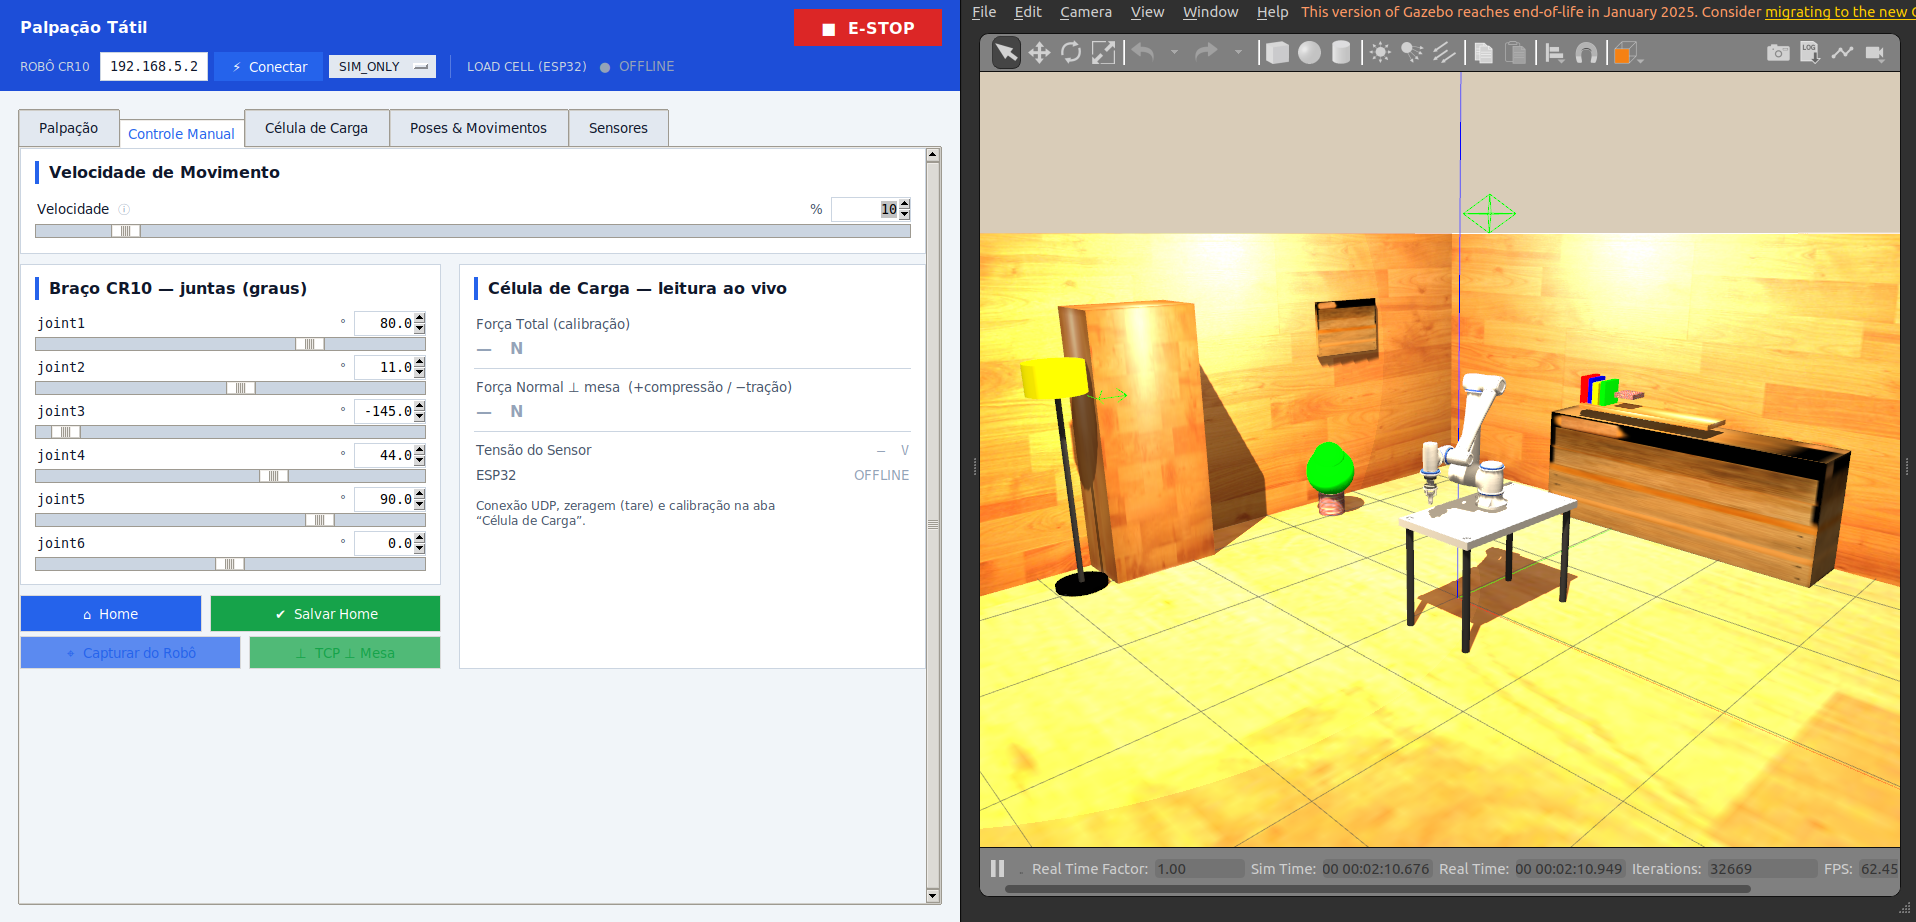
\includegraphics[width=\columnwidth]{touch_pack_gui_manual_gazebo.png}
  \caption{Manual-control view next to the Gazebo twin. The six CR10 joints are
  jogged while the live load-cell reading is displayed; in MIRROR the simulated
  and physical arms move together, so the operator validates motions on the twin
  before they reach the real robot.}
  \label{fig:manual}
\end{figure}

\section{Kinematics and Motion Generation}
\label{sec:kin}
All motion is generated from an analytic forward-kinematics and Jacobian model
of the CR10, expressed directly in the URDF joint convention so that the joint
angles commanded in simulation match those of the physical controller. For a joint vector $q\in\mathbb{R}^6$, forward kinematics yields the
TCP pose $T(q)\in SE(3)$, and the geometric Jacobian $J(q)\in\mathbb{R}^{6\times
6}$ relates joint rates to the TCP twist.

Cartesian motions are realized by streaming joint set points rather than by
planning trajectories offline. At each control tick the task specifies a small
Cartesian step $\Delta\xi=[\,\Delta x^\top\ \Delta\theta^\top]^\top$ (a
translation plus an orientation-locking rotation), and the corresponding joint
increment is obtained with a damped least-squares (DLS) inverse
\cite{nakamura1986,siciliano2009}:
\begin{equation}
\Delta q = J(q)^\top\!\left(J(q)\, J(q)^\top + \lambda^2 I\right)^{-1}\Delta\xi,
\label{eq:dls}
\end{equation}
with damping $\lambda=0.01$ for robustness near singularities. The joint set point
is then $q_{k+1}=q_k+\Delta q$, published with the velocity hint $\Delta q/\Delta
t$. The translational part $\Delta x$ drives the task (approach, slide, retract);
the rotational part $\Delta\theta$ keeps the tool pointing along the approach
axis. Joint set points are clipped to the mechanical limits, and joint velocities
are bounded by a user speed factor (fixed at \SI{10}{\percent} of the rated speed
during palpation for safety).

\section{Palpation Protocol}
\label{sec:fsm}
The palpation cycle is implemented as the finite-state machine (FSM) of
Fig.~\ref{fig:fsm}, reproducing the choreography of \cite{gupta2021} over a
horizontal surface:
\begin{equation*}
\textsc{idle}\!\rightarrow\!\textsc{home}\!\rightarrow\!\textsc{descending}
\!\rightarrow\!\textsc{hold}\!\rightarrow\![\textsc{sliding}]\!\rightarrow\!
\textsc{retract}\!\rightarrow\!\textsc{home}.
\end{equation*}
Every motion phase uses direct set-point streaming at \SI{33}{\hertz}
($\Delta t=\SI{30}{\milli\second}$): each step is computed and published
individually (one point per message, replacing the current goal), so velocity is
bounded explicitly by the step size and no residual motion carries across
phases.

\begin{figure}[t]
  \centering
  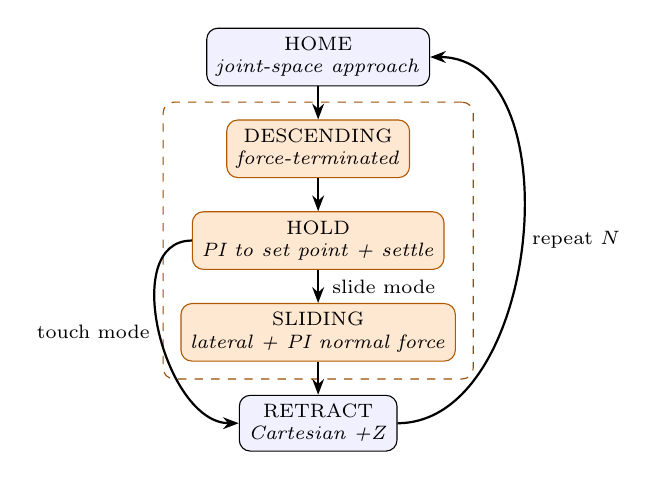
\begin{tikzpicture}[
      font=\scriptsize,
      node distance=4.2mm,
      state/.style={draw, rounded corners, align=center, minimum width=20mm,
                    minimum height=6.0mm, fill=blue!6},
      fstate/.style={state, fill=orange!18, draw=orange!70!black},
      arr/.style={-{Stealth[length=2mm]}, thick}
    ]
    \node[state]  (home)  {HOME\\\textit{joint-space approach}};
    \node[fstate] (desc)  [below=of home] {DESCENDING\\\textit{force-terminated}};
    \node[fstate] (hold)  [below=of desc] {HOLD\\\textit{PI to set point + settle}};
    \node[fstate] (slide) [below=of hold] {SLIDING\\\textit{lateral + PI normal force}};
    \node[state]  (retr)  [below=of slide] {RETRACT\\\textit{Cartesian +Z}};
    \draw[arr] (home) -- (desc);
    \draw[arr] (desc) -- (hold);
    \draw[arr] (hold) -- (slide) node[midway,right=0.5mm]{slide mode};
    \draw[arr] (slide) -- (retr);
    % TOUCH mode shortcut (skip sliding)
    \draw[arr] (hold.west) to[out=180,in=180] node[left]{touch mode} (retr.west);
    % repeat loop
    \draw[arr] (retr.east) to[out=0,in=0] node[right]{repeat $N$} (home.east);
    \begin{scope}[on background layer]
      \node[draw=orange!60!black, dashed, rounded corners, fit=(desc)(hold)(slide),
            inner sep=2.2mm] {};
    \end{scope}
  \end{tikzpicture}
  \caption{Palpation FSM. The three highlighted phases run the closed-loop PI
  normal-force controller (Section~\ref{sec:force}). \textsc{touch} mode skips
  \textsc{sliding} (contact-and-return), while \textsc{slide} mode performs the
  full Gupta cycle; both repeat $N$ times.}
  \label{fig:fsm}
\end{figure}

\textbf{HOME.} A batch joint-space trajectory brings the arm to the start pose at
no more than \SI{0.3}{\radian\per\second} per joint, with the JTC interpolating
an S-curve. The phase verifies that the TCP points downward before contact.

\textbf{DESCENDING.} The tool descends along the approach axis (the tool $-z$
direction) with a fast-to-slow velocity profile, generated by streaming
\eqref{eq:dls}. The phase is \emph{force-terminated}: it ends as soon as the
measured compression reaches the set point. The depth requested in the interface
acts only as a maximum safety stroke.

\textbf{HOLD.} The PI loop drives the compression to the set point and waits for
it to stabilize. Stabilization requires the net contact force $F_k$ to stay within
a tolerance band around the set point $F^\star$ for a continuous interval $T_s$:
\begin{equation}
|F_k - F^\star| \le \max(\tau_a,\, \tau_r F^\star)\quad\text{for } T_s
\text{ continuous},
\label{eq:hold}
\end{equation}
with $\tau_a=\SI{0.15}{\newton}$, $\tau_r=0.05$ (\SI{5}{\percent} of the set point),
$T_s=\SI{1}{\second}$, and a \SI{12}{\second} timeout after which the cycle
proceeds (the slide-phase PI continues to regulate the force).

\textbf{SLIDING} (slide mode only). The tool translates laterally at constant
speed while the PI loop simultaneously regulates the normal force. Orientation,
depth, and the direction perpendicular to the slide are locked so that the PI
acts only along the contact normal. Lateral travel is bounded by a safety limit.

\textbf{RETRACT.} The tool retracts along $+z$ (opposite the approach) by a fixed
distance, after which the cycle either repeats or returns to \textsc{home}.

Two user-selectable modes share this FSM: \textsc{touch} (contact and return,
repeated for a chosen number of touches) and \textsc{slide} (the full cycle with
lateral drag).

\section{Closed-Loop Force Control}
\label{sec:force}
\subsection{Control law}
The contact force is regulated by an outer PI loop (Fig.~\ref{fig:loop}) that maps
the force error to a correction velocity along the approach axis $\hat a$. With
compression positive,
the error at control tick $k$ is
\begin{equation}
e_k = F^\star - F_k,
\label{eq:err}
\end{equation}
where $F^\star$ is the selected set point and $F_k$ the net load-cell reading.
The correction velocity is
\begin{equation}
v_k = g\left(K_p\,e_k + K_i\,I_k + K_d\,\frac{e_k-e_{k-1}}{\Delta t}\right),
\quad
I_k = \mathrm{clip}\!\left(I_{k-1}+g\,e_k\Delta t,\ \pm I_{\max}\right),
\label{eq:pid}
\end{equation}
where $g\in\{0,1\}$ is a contact gate that switches from $0$ to $1$ at first
contact ($F_k>F_c$), suppressing both the output and the integration during the
unloaded approach. The velocity is saturated before use,
$v_k \leftarrow \mathrm{sat}_{\pm v_{\max}}(v_k)$, and the resulting Cartesian
step $\Delta x_k = \hat a\, v_k \Delta t$ is the translational part $\Delta x$ of
\eqref{eq:dls}, producing the joint set point streamed to the controller.

\begin{figure*}[t]
  \centering
  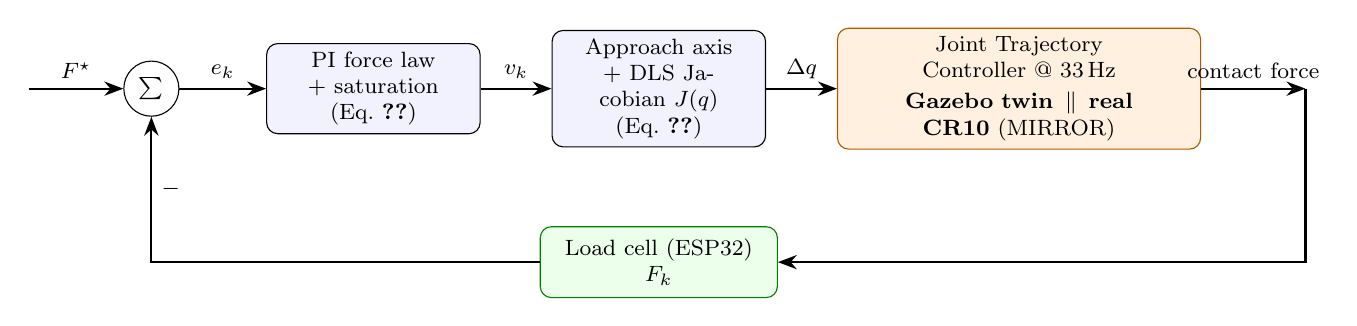
\begin{tikzpicture}[
      font=\footnotesize,
      box/.style={draw, rounded corners, align=center, minimum height=11mm,
                  text width=25mm, fill=blue!5, inner sep=3pt},
      plant/.style={draw, rounded corners, align=center, minimum height=11mm,
                    text width=44mm, fill=orange!12, draw=orange!70!black, inner sep=3pt},
      sens/.style={draw, rounded corners, align=center, minimum height=9mm,
                   text width=28mm, fill=green!8, draw=green!50!black, inner sep=3pt},
      sum/.style={draw, circle, minimum size=7mm, inner sep=0pt},
      arr/.style={-{Stealth[length=2.4mm]}, thick}
    ]
    \node[sum] (sum) {$\sum$};
    \node[box,   right=11mm of sum] (pi)    {PI force law\\$+$ saturation\\(Eq.~\ref{eq:pid})};
    \node[box,   right=9mm of pi]   (dls)   {Approach axis\\$+$ DLS Jacobian $J(q)$\\(Eq.~\ref{eq:dls})};
    \node[plant, right=9mm of dls]  (plant) {Joint Trajectory Controller @ \SI{33}{\hertz}\\[0.6mm]\textbf{Gazebo twin} $\,\Vert\,$ \textbf{real CR10} (MIRROR)};
    \node[right=12mm of plant] (out) {};
    \draw[arr] ([xshift=-12mm]sum.west) -- node[above]{$F^\star$} (sum.west);
    \draw[arr] (sum.east)   -- node[above]{$e_k$}    (pi.west);
    \draw[arr] (pi.east)    -- node[above]{$v_k$}    (dls.west);
    \draw[arr] (dls.east)   -- node[above]{$\Delta q$} (plant.west);
    \draw[arr] (plant.east) -- node[above, align=center]{contact force} (out.center);
    \node[sens, below=10mm of dls] (lc) {Load cell (ESP32)\\$F_k$};
    \draw[arr] (out.center) |- (lc.east);
    \draw[arr] (lc.west) -| (sum.south) node[near end, right]{$-$};
  \end{tikzpicture}
  \caption{Closed-loop force-control architecture (companion to the FSM of
  Fig.~\ref{fig:fsm}). The outer PI loop regulates the normal contact force
  $F_k$, measured by the load cell, to the set point $F^\star$; the resulting
  Cartesian approach velocity $v_k$ is mapped by the damped least-squares
  Jacobian to joint increments $\Delta q$ and streamed at \SI{33}{\hertz}. The plant is
  the \emph{digital twin}: in \textsc{sim\_only} the Gazebo arm, and in
  \textsc{mirror} the Gazebo arm together with the physical CR10, both driven by
  the same set points. The measured joint configuration $q$ closes the
  kinematic feedback into the Jacobian.}
  \label{fig:loop}
\end{figure*}

The integrator is clamped to $\pm I_{\max}$, and the derivative gain is disabled
by default ($K_d=0$), making the nominal controller a PI: the derivative term
amplifies load-cell noise, whereas the physical contact already damps the loop.
The default gains and limits are listed in Table~\ref{tab:params}.

\textbf{Admittance interpretation and tuning.} Equation~\eqref{eq:pid} makes the
tool a velocity source whose speed is proportional to the force error: the
proportional term commands $v=K_p e$, i.e.\ a mechanical \emph{admittance}
$A=K_p$ (meters per second of approach per newton of error), so $K_p$ sets the
contact compliance and $1/K_p$ the effective damping. Against an environment of
stiffness $k_e$, the proportional loop behaves as a first-order response with time
constant $\tau\approx 1/(K_p k_e)$, while the integral term nulls the steady-state
error left by $K_p$ alone. Gains are tuned in this order: $K_p$ for the desired
compliance and settling time given the expected $k_e$, $K_i$ to remove
steady-state error without overshoot, and $K_d=0$.

\textbf{Stability.} Explicit force control of a position-controlled arm against a
stiff environment is prone to contact instability as the product of loop gain and
environment stiffness grows \cite{siciliano2009,villani2016}. Three measures keep
the effective loop gain low in practice: the velocity saturation $v_{\max}$, the
small admittance $K_p$, and the contact gate $g$ that suppresses impact wind-up;
the \SI{10}{\percent} speed factor and the inner trajectory controller further
limit the closed-loop bandwidth, which is in turn bounded by the \SI{33}{\hertz}
control tick. The favorable regime is therefore compliant contact (low $k_e$); on
stiff surfaces $K_p$ must be reduced. A formal passivity analysis and the
bandwidth and stiffness envelope are left as future work.

\begin{table}[t]
  \caption{Control and Safety Parameters (Defaults)}
  \label{tab:params}
  \centering
  \begin{tabular}{@{}lll@{}}
    \toprule
    \textbf{Parameter} & \textbf{Symbol} & \textbf{Value}\\
    \midrule
    Control rate            & $1/\Delta t$ & \SI{33}{\hertz} (\SI{30}{\milli\second})\\
    Proportional gain       & $K_p$        & $1\times10^{-3}$ (m/s)/N\\
    Integral gain           & $K_i$        & $5\times10^{-4}$ (m/s)/(N$\cdot$s)\\
    Derivative gain (PI)    & $K_d$        & $0$\\
    Velocity saturation     & $v_{\max}$   & \SI{5}{\milli\meter\per\second}\\
    Anti-wind-up clamp      & $I_{\max}$   & \SI{5}{\newton\second}\\
    DLS damping             & $\lambda$    & $0.01$\\
    Force set-point limit   & $F^\star_{\max}$ & \SI{10}{\newton}\\
    Force abort limit       & $F_{\mathrm{abort}}$ & \SI{15}{\newton}\\
    Feedback staleness      & $t_{\mathrm{stale}}$ & \SI{0.5}{\second}\\
    \bottomrule
  \end{tabular}
\end{table}

\subsection{Safety layer}
Three independent guards bound the interaction. (i) The set point is saturated to
$F^\star_{\max}=\SI{10}{\newton}$. (ii) If the measured compression exceeds
$F_{\mathrm{abort}}=\SI{15}{\newton}$, the run is aborted and the arm returns
home. (iii) If the load-cell feedback becomes stale (no fresh sample for more
than \SI{0.5}{\second}), all force-controlled phases abort, since regulating
against a frozen reading would drive the tool blindly into the surface. Joint
limits and the \SI{10}{\percent} speed factor provide further kinematic bounds.
On hardware (\textsc{mirror}) the same guards act on the physical arm: the speed
factor is forced to \SI{10}{\percent}, a hardware E-STOP is exposed in the
interface, and the over-force abort retracts the tool, while first-contact
overshoot is limited by the fast-to-slow approach profile and the contact gate.

\section{Experimental Setup}
\label{sec:setup}
The palpation cell is exercised through a graphical interface
(Fig.~\ref{fig:gui}) that exposes the set point, the mode (touch/slide), the
slide speed, distance, and direction, and, under an advanced panel, the PI
gains and the HOLD stabilization parameters. Each run is logged to disk:
per-sample CSV records the relative time, cycle, FSM phase, net force, the six
joint angles, and the TCP position, alongside a JSON of the run parameters and a
per-cycle statistical summary. This logging is the basis of the force-tracking
analysis reported below.

\begin{figure}[t]
  \centering
  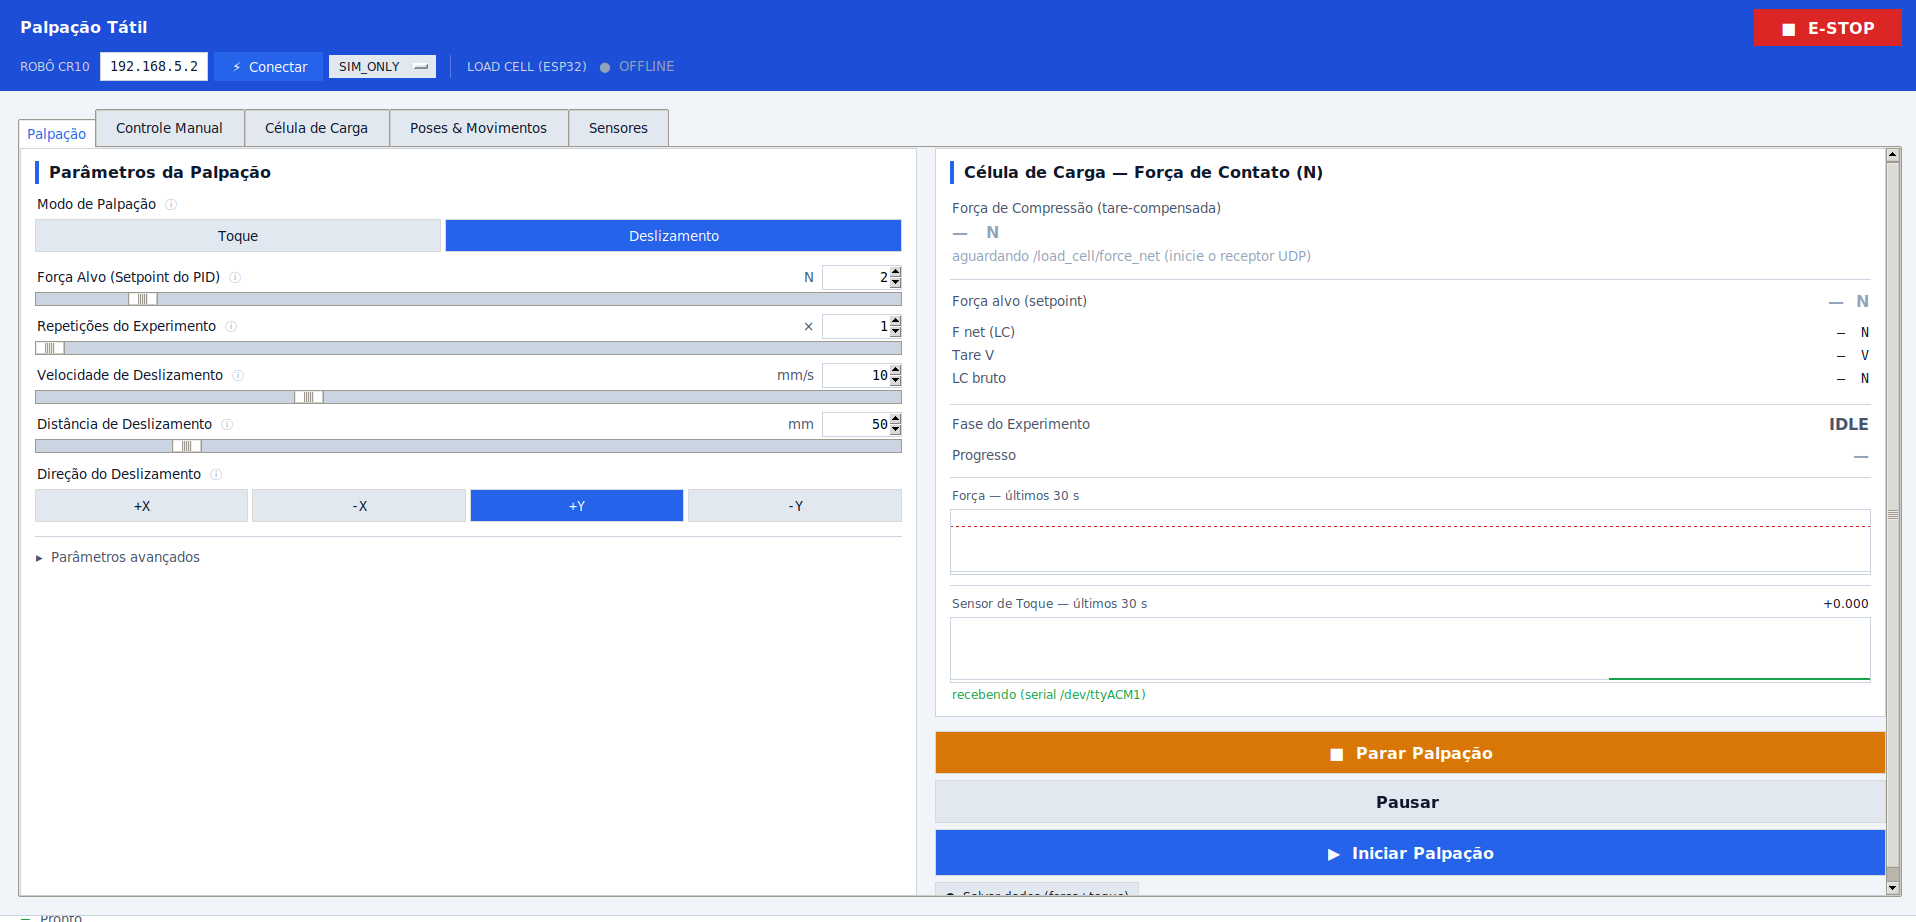
\includegraphics[width=\columnwidth]{touch_pack_gui_palpation_slide.png}
  \caption{Operator interface (slide mode). Left: palpation parameters, force
  set point (PI), repetitions, slide speed, distance, and direction. Right: live
  net contact force from the load cell and the experiment phase. The advanced
  panel (collapsed) exposes the PI gains and the HOLD stabilization band.}
  \label{fig:gui}
\end{figure}

To match \cite{gupta2021}, the protocol is run with the normal force regulated
to set points in the \SIrange{1}{10}{\newton} range and with slide speeds of
$5$, $10$, and \SI{15}{\milli\meter\per\second}. For each configuration we report
the steady-state force error during HOLD, the overshoot during the initial
approach, the time to stabilize \eqref{eq:hold}, and the RMS force error
maintained throughout SLIDING, averaged over repeated cycles. To isolate the
contribution of the integral term, the PI loop is additionally contrasted with a
proportional-only baseline ($K_i=0$).

\section{Results}
\label{sec:results}
\textcolor{red}{\textbf{[PLACEHOLDER: insert the validated arm force-PI data
here.]} Replace Fig.~\ref{fig:results} with the recorded force-tracking plot
(\texttt{figs/pi-force-tracking.png}; the logger already exports a per-run
\texttt{\_\_plot.png}) and fill in Table~\ref{tab:results} with the measured
metrics. Recommended runs: set points of $1$, $2$, $3$, and \SI{5}{\newton} in
\textsc{touch} mode, and a \SI{2}{\newton}, \SI{10}{\milli\meter\per\second},
\SI{50}{\milli\meter} \textsc{slide} run. Suggested narrative: the PI loop drives
the compression to the set point with small overshoot, holds it within the
\eqref{eq:hold} band, and maintains a low RMS force error during the slide.}

\begin{figure}[t]
  \centering
  % When the data is ready, uncomment the line below and delete the framebox.
  % \includegraphics[width=\columnwidth]{pi-force-tracking.png}
  \fbox{\parbox[c][3.6cm][c]{0.93\columnwidth}{\centering\color{red}
  PLACEHOLDER FIGURE\\[2mm]
  Net contact force $F(t)$ vs.\ set point $F^\star$ across the
  DESCENDING / HOLD / SLIDING phases.\\[1mm]
  \footnotesize (Drop the run's \texttt{\_\_plot.png} here.)}}
  \caption{Closed-loop normal-force tracking of the arm. The dashed line is the
  set point $F^\star$; the solid line is the measured net force; shaded bands
  mark the FSM phases. \textcolor{red}{[Replace with recorded data.]}}
  \label{fig:results}
\end{figure}

\begin{table}[t]
  \caption{Force-Tracking Performance (\textcolor{red}{to be filled})}
  \label{tab:results}
  \centering
  \begin{tabular}{@{}lcccc@{}}
    \toprule
    \textbf{Set point} & \textbf{Overshoot} & \textbf{Steady-state} &
    \textbf{Settling} & \textbf{Slide RMS}\\
    $F^\star$ (N) & (\%) & error (N) & time (s) & error (N)\\
    \midrule
    1 & & & & \\
    2 & & & & \\
    3 & & & & \\
    5 & & & & \\
    \bottomrule
  \end{tabular}
\end{table}

\textbf{Qualitative behavior.} Independently of the numbers to be inserted, the
integration is functional end to end: the FSM advances through all phases, the
force-terminated DESCENDING stops at the set point, the HOLD band \eqref{eq:hold}
gates the transition to SLIDING, and the safety guards abort on over-force or
stale feedback. The same control code rehearsed in \textsc{sim\_only} drives the
physical CR10 in \textsc{mirror} without modification.

\section{Discussion}
The digital twin gives three concrete benefits for this task. First,
\emph{safety}: motions are rehearsed in \textsc{sim\_only}, where a collision
costs nothing, and the \SI{15}{\newton} over-force abort and the staleness guard
bound the interaction once contact is made in \textsc{mirror}. Second,
\emph{sim-to-real continuity}: the simulated kinematics is taken from the
manufacturer's URDF and the same control code runs in both worlds, so motions
rehearsed in \textsc{sim\_only} run force-controlled in \textsc{mirror} (where
the real load cell closes the loop) without any code change. Third,
\emph{repeatability}: logged runs make the force-tracking behavior reproducible
and comparable across set points and slide speeds.

The streaming architecture, one set point per tick at \SI{33}{\hertz} with DLS
inverse kinematics, keeps the force loop responsive: corrections take effect
within one control period, and there is no planned trajectory whose momentum must
be overcome when the force loop reacts. The choice of a PI (rather than full PID)
law reflects the noise characteristics of the load cell; the contact itself
supplies the damping that a derivative term would otherwise provide.

\textbf{Limitations.} The load cell measures a single axis, so only the normal
force is regulated; shear during sliding is not directly controlled. The force
loop is layered on position-controlled joints, which bounds the achievable
contact bandwidth. Closing the loop around a tactile sensor, rather than a
single-axis load cell, is left as future work.

\section{Conclusion}
We presented a digital-twin platform of a CR10 collaborative manipulator for
closed-loop, force-controlled tactile palpation. The platform pairs a faithful
ROS~2 / Gazebo simulation with the physical arm through a real-time mirroring
link, and it reproduces the Gupta et al. palpation protocol with a streaming PI
normal-force controller, realized as a tunable admittance, mapped to joint
motion through a damped least-squares Jacobian. The same control code is rehearsed
in simulation and then run, force-controlled, on the physical arm in
\textsc{mirror}, behind a safety layer that bounds interaction forces. Future work
will report the force-tracking accuracy on compliant phantoms with known
stiffness, integrate tactile transduction into the loop, and extend regulation to
shear forces.

\section*{Acknowledgment}
% TODO: advisors, funding agency, institution.
The authors thank \dots

\begin{thebibliography}{00}
% NOTE: verify volume/issue/pages where marked; entries are formatted to IEEE style.
\bibitem{gupta2021} A. K. Gupta, A. Nakagawa, N. F. Lepora, and N. V. Thakor,
``Spatio-temporal encoding improves neuromorphic tactile texture
classification,'' \emph{IEEE Sensors J.}, vol.~21, no.~17, pp.~19038--19046,
Sep.~2021, doi: 10.1109/JSEN.2021.3087511.
\bibitem{konstantinova2014} J. Konstantinova, A. Jiang, K. Althoefer, P.
Dasgupta, and T. Nanayakkara, ``Implementation of tactile sensing for palpation
in robot-assisted minimally invasive surgery: A review,'' \emph{IEEE Sensors
J.}, vol.~14, no.~8, pp.~2490--2501, Aug.~2014.
\bibitem{beccani2014} M. Beccani, C. Di Natali, L. J. Sliker, J. A. Schoen,
M. E. Rentschler, and P. Valdastri, ``Wireless tissue palpation for
intraoperative detection of lumps in soft tissue,'' \emph{IEEE Trans. Biomed.
Eng.}, vol.~61, no.~2, pp.~353--361, Feb.~2014.
\bibitem{siciliano2009} B. Siciliano, L. Sciavicco, L. Villani, and G. Oriolo,
\emph{Robotics: Modelling, Planning and Control}. London, U.K.: Springer, 2009.
\bibitem{nakamura1986} Y. Nakamura and H. Hanafusa, ``Inverse kinematic solutions
with singularity robustness for robot manipulator control,'' \emph{ASME J. Dyn.
Syst., Meas., Control}, vol.~108, no.~3, pp.~163--171, 1986.
\bibitem{hogan1985} N. Hogan, ``Impedance control: An approach to manipulation:
Part I: Theory,'' \emph{ASME J. Dyn. Syst., Meas., Control}, vol.~107, no.~1,
pp.~1--7, 1985.
\bibitem{villani2016} L. Villani and J. De Schutter, ``Force control,'' in
\emph{Springer Handbook of Robotics}, 2nd ed., B. Siciliano and O. Khatib, Eds.
Berlin, Germany: Springer, 2016, pp.~195--220.
\bibitem{macenski2022} S. Macenski, T. Foote, B. Gerkey, C. Lalancette, and W.
Woodall, ``Robot Operating System 2: Design, architecture, and uses in the
wild,'' \emph{Sci. Robot.}, vol.~7, no.~66, eabm6074, 2022.
\bibitem{koenig2004} N. Koenig and A. Howard, ``Design and use paradigms for
Gazebo, an open-source multi-robot simulator,'' in \emph{Proc. IEEE/RSJ Int.
Conf. Intell. Robots Syst. (IROS)}, 2004, pp.~2149--2154.
\bibitem{grieves2017} M. Grieves and J. Vickers, ``Digital twin: Mitigating
unpredictable, undesirable emergent behavior in complex systems,'' in
\emph{Transdisciplinary Perspectives on Complex Systems}. Cham, Switzerland:
Springer, 2017, pp.~85--113.
\bibitem{tao2019} F. Tao, H. Zhang, A. Liu, and A. Y. C. Nee, ``Digital twin in
industry: State-of-the-art,'' \emph{IEEE Trans. Ind. Informat.}, vol.~15, no.~4,
pp.~2405--2415, Apr.~2019.
\bibitem{kritzinger2018} W. Kritzinger, M. Karner, G. Traar, J. Henjes, and
W. Sihn, ``Digital twin in manufacturing: A categorical literature review and
classification,'' \emph{IFAC-PapersOnLine}, vol.~51, no.~11, pp.~1016--1022, 2018.
\bibitem{antfolk2013} C. Antfolk, M. D'Alonzo, B. Ros\'en, G. Lundborg, F.
Sebelius, and C. Cipriani, ``Sensory feedback in upper limb prosthetics,''
\emph{Expert Rev. Med. Devices}, vol.~10, no.~1, pp.~45--54, 2013.
\end{thebibliography}

\end{document}
